\documentclass[12pt,cor2018]{uftpibic}

\usepackage[alf]{abntex2cite}
%\renewcommand{\backrefpagesname}{}
%\renewcommand{\backref}{}
\renewcommand*{\backrefalt}[4]{}

\usepackage{tikz}
\usepackage{multirow}
\graphicspath{{}{images/}{figures/}} 
%-------------------------------------------------------------------------------------------------------------------------%
% Endereço Institucional
%-------------------------------------------------------------------------------------------------------------------------%
\address{109 Norte, Av. Ns 15, ALCNO 14, Bl 04, Sala 207}
\cep{77001-090}
\phone{(63) 3232-8037}
\mail{propesq@uft.edu.br}
\city{Palmas}
%-------------------------------------------------------------------------------------------------------------------------%
% Dados do Projeto
%-------------------------------------------------------------------------------------------------------------------------%
\title{RUTI - Rastreamento Urbano de Transporte Integrado - Fase 2}
\advisor{Prof.}{Tiago da Silva}{Almeida}{Ms.}
\author{}{}
\campus{Campus Universitário de Palmas -- CUP}
\department{Ciência da Computação}
\local{Campus Universitário de Palmas -- CUP, Bloco III, Sala 09}
\area{Ciências Exatas e da Terra}
\financiamento{}
\grupo{GCC -- Grupo de Computação Cientifica}
\keyword{IoT}
\keyword{Transporte Urbano}
\keyword{Rastreamento}
\keyword{Sistemas Embarcados}
\keyword{Aprendizado de Máquina}
\keyword{Reconhecimento de Padrões}
\equipeexecutora{\bf Tiago da Silva Almeida}{\bf Coordenador}
\equipeexecutora{Rafael Lima de Carvalho}{Professor Pesquisador}
\equipeexecutora{Warley Gramacho da Silva}{Professor Pesquisador}
%\equipeexecutora{Leonardo Rezende Costa}{Aluno}
\equipeexecutora{Matheus Aguiar Fagundes}{Aluno}
%-------------------------------------------------------------------------------------------------------------------------%
% Para evitar a quebra automática dos Capítulos, descomentar abaixo
%-------------------------------------------------------------------------------------------------------------------------%
%\makeatletter
%\patchcmd{\chapter}{\if@openright\cleardoublepage\else\clearpage\fi}{}{}{}
%\makeatother
%-------------------------------------------------------------------------------------------------------------------------%
\begin{document}

\maketitle

%\onehalfspacing
\chapter{Introdução}

Grandes centros urbanos trazem grandes desafios à gestão na prestação de serviços de qualidade à população. Um desses desafios é o controle de tráfego devido ao tamanho da frota em grandes centros. Atualmente vivemos uma fase de popularização de projetos que envolvam algum tipo de automação eletrônica. Isso é possível devido aos baixos custos de integração de uma variedades de circuitos acoplados (ou dentro do mesmo encapsulamento, os chamados \textit{System-on-Chip} ou somente SoC), trazendo simplicidade na construção de sistemas automáticos. Logo, surgiu uma linha de pesquisa, chamada \textit{Internet of Things} (IoT), em conjunto com a também simplificada área de desenvolvimento Web. 

As aplicações da metodologia IoT são bastante diversas, podendo ser aplicada também ao controle de tráfego urbano nas grandes cidades. Assim, o objeto desse projeto é desenvolver uma solução baseada em IoT para gerenciamento de frota urbana, especificamente em transporte coletivo. Nosso objetivo é desenvolver um sistema de rastreamento e controle individual de cada veículo, com geolocalização, formar uma base dados em uma aplicação web com os dados dos veículos e também fornecer informações em tempo real aos usuários. 

Os dados capturados dos veículos podem ser utilizados para tomada de decisão em relação a melhores rotas, gastos globais com o transporte, etc.. Um grande desafio, e foco do projeto, é a melhor tecnologia de troca de dados entre veículos e a aplicação Web, devido aos custos de equipamento mais seguros e rápidos e a baixa qualidade da infraestrutura existente. Portanto, nossos esforços empenham-se tanto no sistema de coleta e gestão de dados da frota veicular quanto no desenvolvimento de uma aplicação web (servidor) para gerenciamento dessas informações.

Para completude do projeto é necessários o desenvolvimento de três módulos principais, os quais chamamos de: ``módulo veícular'', ``módulo na estação'' e ``servidor de aplicação''.

Diferente de muitos trabalhos, como o de \citeonline{Barcelos}, o projeto proposto não opera com o padrão IEEE 802.11p. O motivo é que essencialmente o padrão IEEE 802.11p opera sobre frequências muita altas para troca de informação entre veículo e estação, e entre veículo e veículo (entre 5,850 GHz e 5,925 GHz nos Estados Unidos e entre 5,860 GHz e 5,900 GHz na Europa). O que dificulta a aquisição de equipamentos de baixo custo. Entretanto, os módulos propostos se caracterizam como sendo um equipamento previsto no padrão IEEE 802.11p, o OBU (\textit{On Board Unit}) para o módulo veicular e o RSU (\textit{Road Side Unit}) para módulo da estação.

É importante destacar que o trabalho proposto não segue metodologias em camadas como muitos trabalhos da literatura \cite{Moore, Chen}. Isso porque existe o problema da falta de protocolos e arquiteturas padronizadas para criação de projetos caracterizados como IoT, como foi descrito no trabalho de \citeonline{Al-Qaseemi}.

\citeonline{Wang} propuseram um algoritmo cooperativo de controle de semáforos para a rede viária urbana com o objetivo de reduzir o congestionamento de tráfego. As comunicações dedicadas de curto alcance (DSRC - {\it Dedicated Short Range Communications}) são aplicadas para detectar o fluxo de tráfego em tempo real. Com base no fluxo de tráfego no ciclo de semáforos atual e nos dados históricos, foi usada a técnica de aprendizado de máquina para prever a variação do fluxo de tráfego no próximo ciclo de semáforos. Com o objetivo de reduzir o tempo médio de espera da rede rodoviária e equilibrar a pressão de tráfego entre diferentes cruzamentos, o sistema de controle de semáforos ajusta o plano de tempo cooperativamente. Além disso, o algoritmo genético foi usado para calcular o plano ideal de sincronização de semáforos. Além disso, um novo modelo de transição de estados da rede rodoviária para simulação numérica dinâmica é utilizado para verificar a eficácia do algoritmo proposto.

\citeonline{Chen} desenvolveram um modelo para descobrir e visualizar padrões frequentes em registros históricos de resposta a acidentes de trânsito, levando à classificação automática de níveis de severidade entre incidentes passados usando aprendizado de máquina avançado e aprendizado ativo. Os experimentos foram executados usando registros de incidentes de 4 anos da TMC ({\it Transport Management Centre}) de 2011 a 2014 em Sidney, Austrália, o que inclui mais 40.000 registros. O modelo de classificação alcançou quase 90\% de precisão em cinco vezes a validação cruzada e espera-se que ajude o TMC a melhorar seus procedimentos, planos de resposta e alocação de recursos.

O trabalho de \citeonline{Fadlullah} é uma referência importante para esse projeto, pois demonstra a necessidade de pesquisar os trabalhos dispersos em aplicativos de aprendizagem profunda para vários aspectos de controle de tráfego de rede de computadores. Além disso, fornece uma visão geral das arquiteturas e algoritmos de aprendizagem profunda de última geração relevantes para os sistemas de controle de tráfego de rede, discutindo os facilitadores de aprendizado profundo para sistemas de rede, além de uma série de questões de pesquisa aberta, que os pesquisadores podem considerar úteis no futuro, que é nosso caso.

Destacado isso, o objetivo é desenvolver uma arquitetura simplificada para troca de informação com menor latência. Ou seja, os módulos terão somente duas camadas: uma camada abstrata de aplicação e uma camada abstrata de coleta de dados, sem referência com o modelo OSI (\textit{Open System Interconnection}). 

\chapter{Objetivos}

O objetivo deste projeto é desenvolver um servidor de aplicação para os dados coletados dos módulos desenvolvidos na primeira fase do projeto e junto com um algoritmo de aprendizado de máquina para reconhecimento de padrões de utilização do transporte coletivo para proposição de melhores formas de utilização de acordo com a demanda. Os objetivos de pesquisa podem ser detalhados da seguinte forma:

\begin{itemize}
\item Desenvolvimento de uma base de dados;
\item Desenvolvimento de uma aplicação web para manipulação dos dados coletados;
\item Integração do servidor web com os módulos desenvolvidos na primeira fase do projeto;
\item Aplicação e desenvolvimento de algoritmo de aprendizado de máquina;
\item Coleta de dados em ambiente controlado;
\item Reconhecimento dos padrões de utilização do transporte coletivo;
\item Análise estatística dos resultados.
\end{itemize}

%Como processador, ou como gerenciador, do módulo existem várias opções, como Raspberry \cite{raspberry} ou Photon \cite{photon}. Mas por simplicidade, custo e documentação, será utilizado no projeto a plataforma Arduino \cite{arduino}.

\chapter{Metodologia}

Nesta seção será explicado o projeto como um todo, destacando inclusive as partes que compões a primeira etapa do projeto. Contudo, a segunda fase tem o foco no desenvolvimento do servidor de aplicação com aprendizado de máquina para que haja o reconhecimento de padrões de utilização dos usuários do transporte público, bem como a criação de rotas e horários de utilização com base nessa base de conhecimento. Assim, haverá um estudo detalhado sobre a utilização e funcionamento das técnicas de aprendizado de máquina para que o servidor seja autossuficiente nesse reconhecimento.

Na primeira fase do projeto são utilizadas plataformas microcontroladas para gerenciamento da comunicação de dados. Atualmente diversas plataformas baseadas em microcontroladores e SoCs são empregadas em projeto de IoT, e em sua maioria são de código fonte aberto. Por possuir um custo baixo e ampla documentação, escolhemos a plataforma Arduino. A Figura \ref{fig:projeto1} e \ref{fig:projeto2}, ilustra todas os componentes do projeto, destacado os módulos que serão desenvolvidos em pontilhado, e as interações entre esses componentes focando no módulo veicular (Figura \ref{fig:projeto1}) e no módulo da estação (Figura \ref{fig:projeto2}). O módulo na estação é um nó secundário da rede de comunicação, gerenciado também por um microcontrolador. Secundário porque o módulo será usado para correção e sincronismo do módulo acoplado ao veículo.

\begin{figure}[!htpb]
\centering
\caption{Diagrama de fluxo de dados do módulo veicular, destacando os sub-módulos envolvidos e os canais de comunicação em cada etapa.}
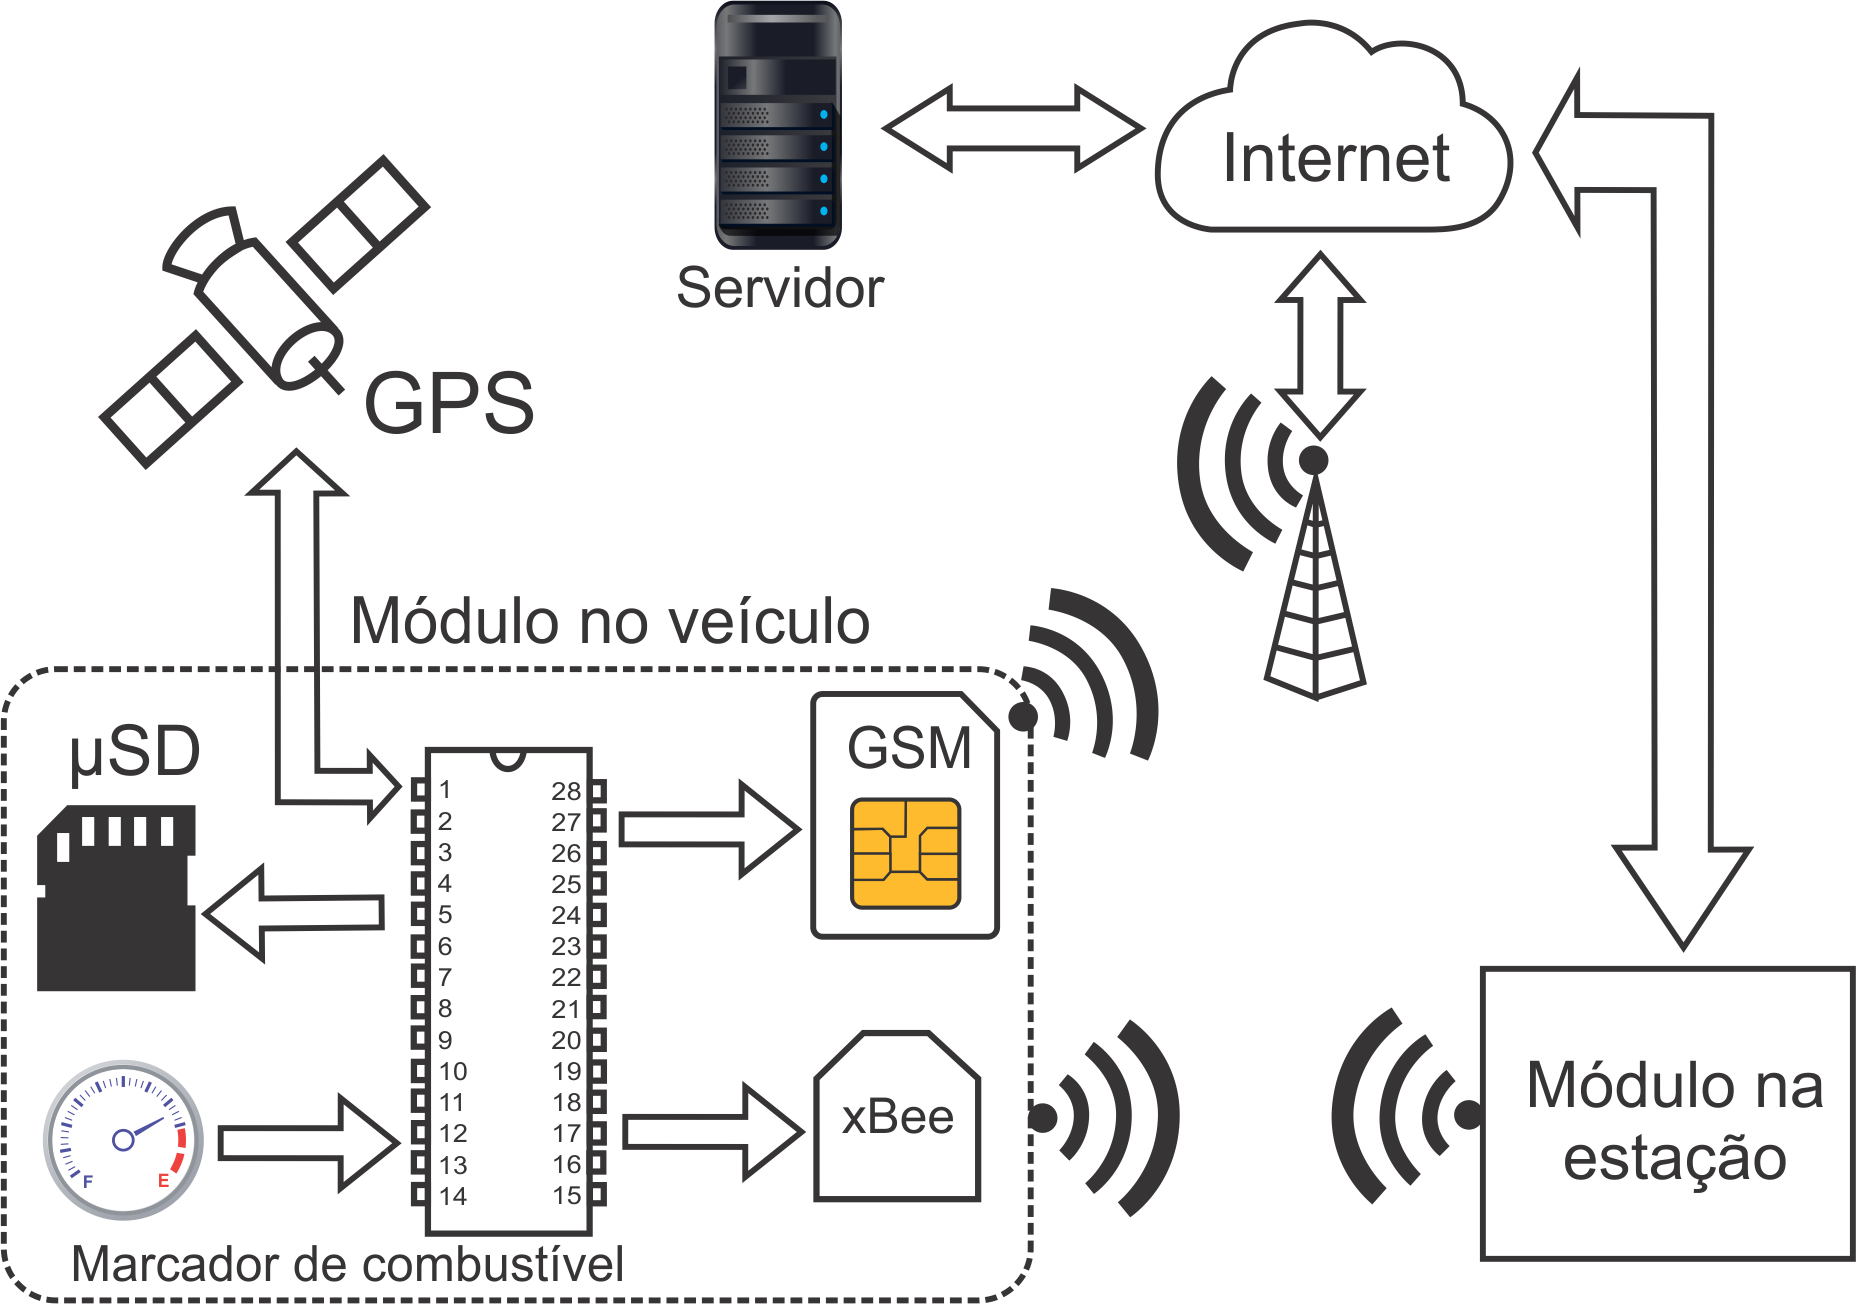
\includegraphics[scale=.8]{ruti1.png}
\label{fig:projeto1}
\end{figure}

O módulo no veículo é o nó central da rede de comunicação sendo gereanciado pelo microcontrolador. Acoplado ao microcontrolador existem três sub-módulos principais para comunicação externa, todos sem o uso de fios. 

A primeiro é formado pelo sub-módulo GPS que verifica a posição do veículo, em termos de latitude e longitude, e velocidade. Portanto, esse sub-módulo está presente somente no módulo veicular. O sub-módulo GPS faz a comunicação direta com o satélite, logo, a comunicação nesse ponto é externa ao modelo veicular dentro do nosso projeto. 

O segundo sub-módulo é forma pela comunicação GSM, com foco na rede de dados fornecida pelas operadoras de celulares. O objetivo desse sub-módulo é somente enviar as informações do veículo para um servidor na internet. Essa comunicação é de vital importância para criação de uma base de dados robusta para explorar a análise de tráfego e utilização do transporte público em trabalhos futuros.

\begin{figure}[!htpb]
\centering
\caption{Diagrama de fluxo de dados do módula na estação, destacando os sub-módulos envolvidos e os canais de comunicação em cada etapa.}
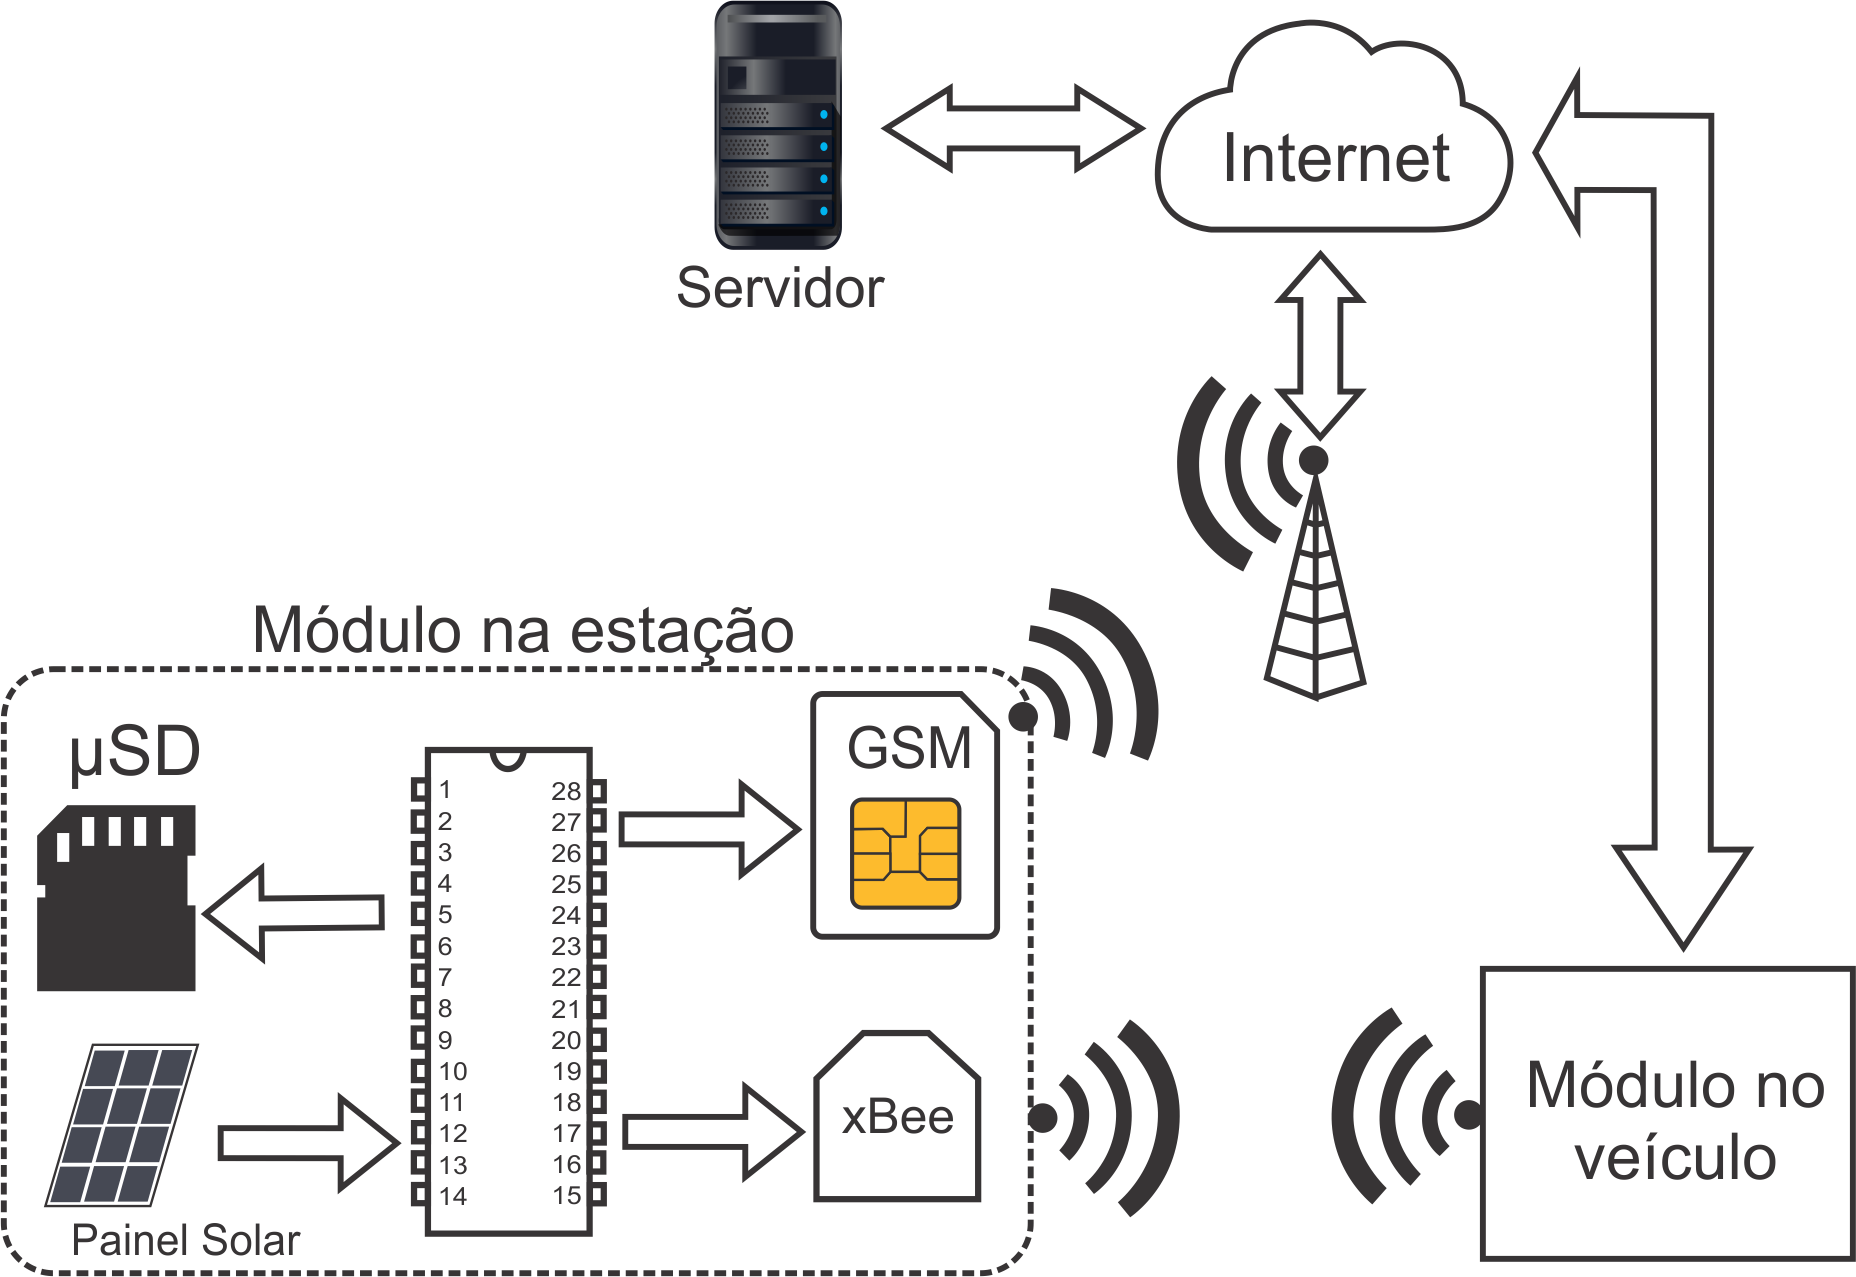
\includegraphics[scale=.8]{ruti2.png}
\label{fig:projeto2}
\end{figure}

O terceiro sub-módulo de comunicação será utilizada a comunicação baseado no padrão IEEE 802.15.4, popularmente conhecido com ``ZigBee'' \cite{Hoang}. O padrão IEEE 802.15.4 funciona com altas frequências de operação, comparado à sinais mais comuns como rádio frequência, e baixa taxa de transferência de dados. Objetivo é fornecer um protocolo seguro e redundante para manter a integridade dos dados na comunicação. O terceiro sub-módulo será usado na comunicação com a estação ou ponto de ônibus e locais de maior fluxo. Como o sub-módulo GPS e GSM possuem latências altas de resposta devido a problemas de infraestrutura, o módulo ZigBee fornece os dados ao módulo na estação e a estação reenvia e ajusta o sincronismo na linha, de modo a permitir que as dados no servidor sejam em tempo real.

Além dos sub-módulos de comunicação externa, o módulo do veículo (Figura \ref{fig:projeto1}) conta com um leitor de cartão de memória, que funcionará como \textit{datalogger}, salvando as informações em caso de falha de comunicação ou outro tipo de falha no veículo e um leitor do nível de combustível, como por exemplo no trabalho de \citeonline{Lozoya}. Como veículos antigos não possuem computador de bordo, o sub-módulo proposto nesse projeto funcionará como sendo um e será de fácil adaptação já que os medidores de combustível são sensores do tipo boia dentro do tampo ligado a uma resistência elétrica, e por essa variação de resistividade é dado no painel a quantidade de combustível no tanque. Essa característica permite o acoplamento do módulo proposto sem grandes transtornos. A implementação pode ser feita, se baseando no trabalho de \citeonline{Xu}.

Outro ponto importante é a necessidade de adequar o consumo de energia dos componentes, uma vez que os módulos precisarão ter certa autonomia e não necessariamente funcionará conectado à rede elétrica. Esse é um trabalho que deverá ser feito em fluxo contínuo ao longo do desenvolvimento dos protótipos propostos nesse trabalho.

Na segunda fase do projeto, o qual esse projeto de iniciação científica foca, refere-se ao servidor de aplicação onde os dados são armazenados (Figura \ref{fig:projeto1} e \ref{fig:projeto2}, ``servidor''). A base de dados é formada pelas técnicas convencionais de banco de dados relacional, juntamente com uma aplicação web, também com técnicas convencionais de desenvolvimento de aplicações web. O ponto central é o aprendizado de máquina para o ``tratamento'' dos dados, de modo que o sistema evolua para outras formas de rotas a partir dos padrões descobertos com a utilização e coleta dos dados da primeira fase.

Além do aprendizado de máquina, existe o chamado aprendizado profundo é um ramo do aprendizado de máquina baseado em um conjunto de algoritmos, que constroem modelos computacionais com o objetivo de representar abstrações de dados de alto nível. Na literatura, a aprendizagem profunda também tem sido referenciada como aprendizagem profundamente estruturada, aprendizagem hierárquica, aprendizagem profunda e representação profunda \cite{Fadlullah}. 

\chapter{Cronograma de execução}

As atividades do trabalho são divididas conforme a Tabela \ref{tb:atividades}, enumeradas de A à J, e sua execução é de acordo com o cronograma da Tabela \ref{tb:cronograma}.

\begin{table}[!h]
  \centering
  \caption{Lista de atividades previstas.}\label{tb:atividades}
  \begin{tabular}{cp{9.4cm}}
    \hline \hline &\\[-0.4cm]
    {\bf Atividades} & \multicolumn{1}{c}{\bf Descrição} \\
    \hline
    &\\[-0.4cm]
    \textbf{A} &  Desenvolvimento de uma base de dados. \\[0.2cm]
    \textbf{B} &  Desenvolvimento de uma aplicação web para manipulação dos dados coletados.\\[0.2cm]
    \textbf{C} &  Integração do servidor web com os módulos desenvolvidos na primeira fase do projeto.\\[0.2cm]
    \textbf{D} &  Estudo dos algoritmos de aprendizado de máquina. \\[0.2cm]
    \textbf{E} &  Aplicação e desenvolvimento de algoritmo de aprendizado de máquina. \\[0.2cm]
    \textbf{F} &  Coleta de dados em ambiente controlado.\\[0.2cm]
    \textbf{G} &  Reconhecimento dos padrões de utilização do transporte coletivo.\\[0.2cm]
    \textbf{H} & Análise estatística dos resultados. \\[0.2cm]
    \textbf{I} &  Escrita de relatório parcial em forma de trabalhos parciais para publicação em congressos e/ou periódicos e como relatório de prestação de contas com os sistemas de gestão da UFT. \\[0.2cm]
    \textbf{J} &  Escrita de relatório final em forma de trabalhos parciais para publicação em congressos e/ou periódicos e como relatório de prestação de contas com os sistemas de gestão da UFT. \\[0.2cm]
    \hline \hline
  \end{tabular}
\end{table}


\begin{table}[!ht]
  \centering %\fontsize{8}{12}%\tiny
  \caption{Cronograma de Atividades.}\label{tb:cronograma}
  \begin{tabular}{|c|c|c|c|c|c|c|c|c|c|c|c|c|}
    \hline
    {\normalsize\bf Ano}  &\multicolumn{12}{c|}{\normalsize\bf 2018/2019}\\
    \hline
 {\normalsize\bf Mês} &
\multirow{2}*{\bf Jul}&\multirow{2}*{\bf Ago}&\multirow{2}*{\bf Set}&\multirow{2}*{\bf Out}&\multirow{2}*{\bf Nov}&\multirow{2}*{\bf Dez}&
\multirow{2}*{\bf Jan}&\multirow{2}*{\bf Fev}&\multirow{2}*{\bf Mar}&\multirow{2}*{\bf Abr}&\multirow{2}*{\bf Mai}&\multirow{2}*{\bf Jun} \\
   \cline{1-1}
{\bf Atv.}    & & & & & & & & & & & &   \\
\hline
{\normalsize\bf A} & $\surd$ & $\surd$ & & & & & & & & & &  \\
\hline
{\normalsize\bf B} & & $\surd$ & $\surd$ & $\surd$ & $\surd$ & $\surd$ & $\surd$ & & & & & \\
\hline
%\hhline{>{\arrayrulecolor{black}}---->{\arrayrulecolor{black}}->{\arrayrulecolor{black}}------}
{\normalsize\bf C} & & & $\surd$ & $\surd$ & $\surd$ & $\surd$ & & & & & &  \\
%\hhline{>{\arrayrulecolor{black}}----->{\arrayrulecolor{black}}-->{\arrayrulecolor{black}}----}
\hline
{\normalsize\bf D} & & & & & $\surd$ & $\surd$ & $\surd$ & $\surd$ & $\surd$ & & &  \\
%\hhline{>{\arrayrulecolor{black}}------>{\arrayrulecolor{black}}->{\arrayrulecolor{black}}----}
\hline
{\normalsize\bf E} & & & & & & $\surd$ & $\surd$ & $\surd$ & $\surd$ & $\surd$ & &  \\
%\hhline{>{\arrayrulecolor{black}}------->{\arrayrulecolor{black}}->{\arrayrulecolor{black}}---}
\hline
{\normalsize\bf F} & & & & & & & $\surd$ & $\surd$ & $\surd$ & $\surd$ & $\surd$ & \\
% \hhline{>{\arrayrulecolor{black}}-------->{\arrayrulecolor{black}}-->{\arrayrulecolor{black}}-}
\hline
{\normalsize\bf G} & & & & & & & & & $\surd$ & $\surd$ & $\surd$ &  \\
% \hhline{>{\arrayrulecolor{black}}-------->{\arrayrulecolor{black}}-->{\arrayrulecolor{black}}-}
\hline
{\normalsize\bf H} & & & & & & & & & & $\surd$ & $\surd$ & \\
% \hhline{>{\arrayrulecolor{black}}-------->{\arrayrulecolor{black}}-->{\arrayrulecolor{black}}-}
\hline
{\normalsize\bf I} & & & & & & $\surd$ & $\surd$ & &  & & &  \\
\hline

{\normalsize\bf J} & & & & & & & & & & & $\surd$ & $\surd$ \\
\hline
  \end{tabular}
\end{table}

{\color{white}
texto

texto

texto

texto

texto

texto

texto

texto

texto

texto
}

\chapter{Resultados esperados}

Ao final do projeto, esperamos que haja um protótipo para o módulo na estação e um para o módulo no veiculo para coleta de dados e já existam dados suficientes para a disponibilidade e tratamento dos dados, os quais poderão ser empregados em algoritmos de aprendizado de máquina para análise de tráfego e utilização do transporte coletivo.

Com o modelo proposto de coleta e tratamento dos dados de tráfego de transporte público, esperamos que seja fácil à implementação em qualquer grande centro urbano o qual sofra de problemas com transporte público. A utilização do aprendizado de máquina faz que o sistema ``aprenda'' as características de cada local apresente soluções específicas para cada caso.


\bibliography{bibliografia}

\end{document}

